\documentclass{report}
\usepackage[margin=1in, paperwidth=8.5in, paperheight=11in]{geometry}
%Math packages%
\usepackage{amsmath}
\usepackage{amssymb}
\usepackage{amsthm}
%Spacing%
\usepackage{setspace}
\onehalfspacing
%Lecture number%
\newcommand{\lectureNum}{17}
%Variables - Date and Course%
\newcommand{\curDate}{February 10, 2017}
\newcommand{\course}{MATH 239}
\newcommand{\instructor}{Luke Postle}
%Defining the example tag%
%\theoremstyle{definition}%
\newtheorem{ex}{Example}[section]
%Setting counter given the lecture number%
\setcounter{chapter}{\lectureNum{}}
%Package for drawing graphs%
\usepackage{tikz}
\usepackage{verbatim}
\usetikzlibrary{arrows}

\begin{document}
%Note title%
\begin{center}
\begin{Large}
\textsc{\course{} | Lecture \lectureNum{}}
\end{Large}
\end{center} 
\noindent \textit{Bartosz Antczak} \hfill
\textit{Instructor: \instructor{}} \hfill
\textit{\curDate{}}
\rule{\textwidth}{0.4pt}
\section{More on Colouring}
\subsubsection{Definition | D-degenerate}
A graph $G$ is \textbf{d-degenerate} is every subgraph $H$ of $G$ has a vertex of degree at most $d$ in $H$.
\begin{ex}
Consider the following graph. The max degree found in every subgraph H of G is at most 3 (observe that there is a vertex of degree 4, but this vertex isn't found in \underline{every} subgraph).
\end{ex}
%Example 1%
\begin{center}
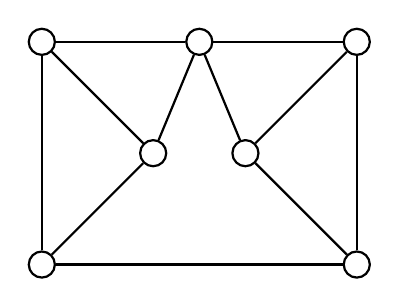
\begin{tikzpicture}[-,auto,node distance=2cm,
                    thick,main node/.style={circle,draw,font=\sffamily\small}]

  \node[main node] (1) {};
  \node[main node] (3) [right of=1] {};
  \node[main node] (2) [left of=1] {};
  \node[main node] (4) [below left of=3] {};
  \node[main node] (5) [below right of=2] {};  
  \node[main node] (6) [below left of=5] {};
  \node[main node] (7) [below right of=4] {};  
  
  \path[every node/.style={font=\sffamily\large}]
    (1) edge (2)
    	edge (3)
    	edge (4)
    	edge (5)
    (5) edge (2)
    	edge (6)
    (4) edge (3)
    	edge (7)
    (7) edge (3)
    (6) edge (7)
    	edge (2);
\end{tikzpicture}
\end{center}
An equivalent formulation is:
\begin{center}
$G$ is \textbf{d-degenerate} if there exists an ordering $v_1, v_2, \cdots, v_n \in V(G)$ such that for all $i$, the number of neighbours of $v_i$ with index $< i$ is at most $d$.
\end{center}
These definitions are equivalent. 
\subsection{Lemma 1} (Will be useful for the homework)
\begin{center}
\textit{If G is $d-$degenerate, then G is $(d+1)-$colourable}
\end{center}
\subsubsection{Proof of Lemma 1}
Since $G$ is $d-$degenerate, there exists an ordering $v_1, \cdots, v_n$ as outlined in the definition previously mentioned. Now colour the vertices of $G$ in that order, giving $v_i$ the lowest colour in $\{1, \cdots, d+1\}$ not used by its earlier neighbours. Thus, we have $d+1$ colours.
\subsection{Question 1}
\begin{center}
How many colours (in the worst case) do you need to colour a planar graph? More formally, which is the maximum value of $\chi(G)$ for all planar $G$?
\end{center}
\subsection{Theorem 1 (6 colour theorem)}
\begin{center}
\textit{If G is a planar graph, then G is 6-colourable}
\end{center}
This follows from our next lemma, combined with Lemma 1.
\subsection{Lemma 2}
\begin{center}
\textit{If G is planar, then G is 5-degenerate}
\end{center}
\subsubsection{Proof of Lemma 2}
Let $H$ be a subgraph of $G$. Since $G$ is planar, then $H$ is planar. By our corollary of Euler's formula, $$|E(H)| \leq 3|V(H)| - 6$$ By the Handshaking lemma $$\sum_{v\in V(H)} \mathrm{deg}(v) = 2|E(H)| \leq 6|V(H)| - 12$$
Thus, there exists a vertex of $H$ of degree at most 5, otherwise, there exists a degree of at least 6, which means that $\displaystyle \sum_{v \in V(H)} \mathrm{deg}(v) \geq 6|V(H)|$, which is a contradiction.
\subsubsection{Definition | Contraction}
If $e = uv$ is an edge of $G$, then the \textbf{contraction} of $e$, denoted $G / e$ is the graph where we delete $u$ and $v$ and add a new vertex $w$ adjacent to all of $N(u) \cup N(v)$ ($N$ denotes the neighbours of the current vertex).
\begin{ex}
A contracted graph
\end{ex}
\begin{center}
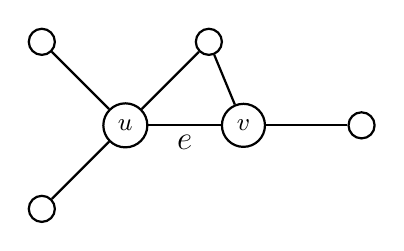
\begin{tikzpicture}[-,auto,node distance=1.5cm,
                    thick,main node/.style={circle,draw,font=\sffamily\small}]

  \node[main node] (1) {};
  \node[main node] (2) [below right of=1] {$u$};
  \node[main node] (3) [below left of=2] {};
  \node[main node] (4) [above right of=2] {};
  \node[main node] (5) [right of=2] {$v$};  
  \node[main node] (6) [right of=5] {};
  
  \path[every node/.style={font=\sffamily\large}]
    (2) edge (1)
    	edge (3)
    	edge (4)
    	edge node [below] {$e$} (5)
    (5) edge (6)
    	edge (4);
\end{tikzpicture}
$\qquad\qquad \implies \qquad\qquad$
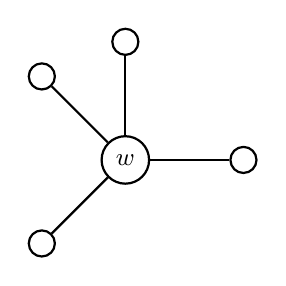
\begin{tikzpicture}[-,auto,node distance=1.5cm,
                    thick,main node/.style={circle,draw,font=\sffamily\small}]

  \node[main node] (1) {};
  \node[main node] (2) [below right of=1] {$w$};
  \node[main node] (3) [below left of=2] {};
  \node[main node] (4) [above of=2] {};
  \node[main node] (5) [right of=2] {};
  
  \path[every node/.style={font=\sffamily\large}]
    (2) edge (1)
    	edge (3)
    	edge (4)
    	edge (5)
    	edge (4);
\end{tikzpicture}
\end{center}

\subsection{Proposition 1}
\begin{center}
\textit{If G is a planar graph and $e \in E(G)$, then $G/e$ is planar}
\end{center}
Proof is left as an exercise to the reader.
\subsection{5-colour Theorem}
\begin{center}
\textit{If G is planar, then G is 5-colourable}
\end{center}
\subsubsection{Proof of 5-colour Theorem}
We proceed by induction on $|V(G)|$. By our lemma, $G$ is 5-degenerate and so has a vertex $v$ of at most 5. Consider two cases:
\begin{itemize}
\item $\mathrm{deg}(v) \leq 4$: then colour $G-v$ with a 5-colouring by induction. Then extend the colouring to $v$ by giving $v$ a colour different from all of its neighbour's colours. This is possible because $v$ has at most 4 neighbours and we have at least 5 colours.
\item $\mathrm{deg}(v) = 5$: let $x, y$ be non-adjacent neighbours of $v$. Note, such $x,y$ exist as otherwise, $N(v) = K_5$, contradicting that $G$ is planar. Now let $G^\prime = G / e_{\{vx, vy\}}$ (i.e., contract two edges). Let $z$ be the new vertex in place of $x,v,y$ whose neighbourhood in $G^\prime$ is $N(x) \cup N(y) \cup N(v) - \{v,x,y\}$.\\By our proposition, $G^\prime$ is planar. Yet, $|V(G^\prime)| \leq |V(G)|$, thus my induction, $G^\prime$ has a 5-colouring. Now we extend this colouring to $G$ by:
\begin{itemize}
\item colouring both $x$ and $y$ with the colour of $z$, then
\item colour $v$ with a colour not used by its neighbours. This works because we have at most 5 neighbours but two ($x$ and $y$) have the \underline{same} colour.
\end{itemize}
\end{itemize}
In fact, we can go even deeper. A planar graph can be in fact \textbf{4-colourable}.
%END%
\end{document}